%----------------------------------------------------------
% PACKAGES AND THEMES
%----------------------------------------------------------
\documentclass[aspectratio=169,xcolor=dvipsnames,handout]{beamer}

\usetheme{Darmstadt}
\usecolortheme{seahorse}

\usepackage[hangul]{kotex}
\usepackage{hyperref}
\usepackage{graphicx, array, adjustbox, makecell}
\usepackage{booktabs, multicol, multirow}
\setbeamercovered{transparent}

%----------------------------------------------------------
% TITLE PAGE
%----------------------------------------------------------
\title{단체교섭}
\subtitle{노사관계의 이론과 실제}
\author{오성재}
\institute[CNU]
{\relax
    충남대학교 경제학과\\
}
\date{2024년 9월 25일}

%----------------------------------------------------------
\begin{document}
%----------------------------------------------------------

\frame{\titlepage}

\begin{frame}{목차}
    \small
    %아래 둘 중 하나만 쓸 것
    \tableofcontents[hideallsubsections]
    %\tableofcontents
\end{frame}

\section{단체교섭의 의의}

\begin{frame}[allowframebreaks]{기능과 성격}
    \begin{block}{단체교섭 (collective bargaining)}
        \begin{itemize}[<+->]
        \item 피고용인들이 노동조합이라는 교섭력을 바탕으로 임금, 근로조건의 유지·개선과 복지증진 및 경제적·사회적 지위향상을 위해 사용자와 교섭하는 것
        \end{itemize}
    \end{block}
    \begin{itemize}[<+->]
        \item 노사가 대등한 입장에서 협상과 타협을 통하여 근로조건을 결정하는 단체교섭은 노동조합의 가장 중요한 기능이며, 집단고용관계의 핵심
        \item 단체교섭의 기본적인 기능
            \begin{itemize}[<+->]
                \item 피고용인의 작업장 규칙을 제정하고 수정하는 기능
                \item 피고용인의 보상의 양을 결정하는 기능
                \item 분규를 해결하는 방법을 제공하는 기능
            \end{itemize}
        \framebreak\relax
        \item 단체교섭의 성격
            \begin{itemize}[<+->]
                \item 노동조합과 사용자대표 간의 쌍방적 결정
                \item 단체교섭은 그 자체가 목적이나 귀결점이 아닌 과정
                \item 노사 쌍방이 다양한 수단과 방법을 동원하여 타결점을 찾는 일련의 정치적 과정
                \item 상호 신의에 따라 성실히 교섭하여 협약이 체결되도록 노력: 노사 양측에 성실교섭의무 부과
            \end{itemize}
    \end{itemize}
\end{frame}

\begin{frame}{피고용인과 기업경영에의 영향}
    \begin{itemize}[<+->]
        \item 단체교섭이 근로자와 경영자에 주는 영향
        \begin{itemize}[<+->]
            \item 노동조건을 통일적으로 형성하는 역할
            \item 피고용인의 욕구불만을 조정하는 역할: 이 역할이 제대로 이루어지지 않으면 사기 저하, 결근 또는 이직 등과 같은 다양한 형태의 불만 (silent strikes)이 표출됨
            \item 경영에 제 분야를 압박·자극하여 전문화를 유도하는 기능. 예를 들어 무노조 기업에서 노조가 결성되면 경영이 보다 전문화되는 경향이 존재 (shock effect)
            \item 사회전체 고용관계의 패턴을 정하는 역할 (pattern setter)
        \end{itemize}
    \end{itemize}
\end{frame}

\section{목표, 주체, 대상 및 구분}

\begin{frame}{노사 당사자의 교섭 목표}
    \begin{itemize}[<+->]
        \item 노동조합의 교섭 목표: 노동의 대가를 노동자에게 유리하게 교섭·결정
        \begin{itemize}[<+->]
            \item 노동조건, 특히 임금·노동시간 등의 교섭을
        \end{itemize}
            \item 사용자측의 단체교섭 목표: 주주나 기업주에게 투자한 데 대한 충분한 보상 확보
        \begin{itemize}[<+->]
            \item 노동조합과의 각종 교섭에서 합리적이고 적절한 수준에서 협상 타결을 위해 노력
            \item 기업의 지속적인 성장 유지
        \end{itemize}
    \end{itemize}
\end{frame}

\begin{frame}[allowframebreaks]{당사자 및 담당자}
    \begin{itemize}[<+->]
        \item 당사자: 단체교섭 결과 단체협약이 체결되는 경우 협약상의 권리·의무의 주체가 되는 자
        \begin{itemize}[<+->]
            \item 근로자측 단체교섭 당사자: 개별 근로자에게 권리로 보장되었으나 실제는 노동조합이 됨
            \item 사용자측 단체교섭 당사자: 근로계약에 의해 근로자를 채용한 계약상의 당사자인 사용자 (및 단체)
        \end{itemize}
    \framebreak\relax
    \item 담당자: 단체교섭을 직접적으로 담당하는 자
        \begin{itemize}[<+->]
            \item 노동조합측의 교섭 담당자: 교섭방식에 따라 상이
        \begin{itemize}[<+->]
            \item 기업별 교섭: 단위 노조의 대표자 및 교섭위원으로 지명된 조합원
            \item 집단교섭: 단위노동조합의 대표자 중에서 선정된 자
            \item 산업별· 대각선 교섭: 단위노동조합으로부터 위임을 받은 연합노동조합의 대표자
        \end{itemize}
    \item 사용자측의 교섭담당자: 사용자나 사용자로부터 위임 받은 지배인·사용자단체 대표자, 사용자단체가 자체 정관으로 지정한 자 등
        \end{itemize}
    \end{itemize}
\end{frame}

\begin{frame}[allowframebreaks]{단체교섭 대상}
    \begin{enumerate}[<+->]
        \item 의무적 교섭사항
        \begin{itemize}[<+->]
            \item 근로자의 권리로 보장되고 사용자의 의무로 되어 있는 사항
            \item 사용자가 거부 또는 성실히 교섭하지 않을 경우 부당노동행위
            \begin{itemize}[<+->]
                \item 근로자의 노동조건 등과 관련성이 있는 사항
                \item 노동조합과 단체협상에 관련된 사항
                \item 경영상 불가피 하고 근로자의 이해와 직접 관련된 사항
            \end{itemize}
        \end{itemize}
    \framebreak\relax
    \item 임의적 교섭사항
        \begin{itemize}[<+->]
            \item 근로자의 요구에 따라 단체교섭을 할 수 있는 사항
            \item 사용자가 거부 또는 성실히 교섭하지 않을 경우 부당노동행위가 성립되지 않음
            \begin{itemize}[<+->]
                \item 인사권·경영권·영업양도·회사조직변경 등
            \end{itemize}
        \end{itemize}
    \item 불법적 교섭사항
        \begin{itemize}[<+->]
            \item 교섭자체가 불법이므로 교섭의무가 존재하지 않음
            \begin{itemize}[<+->]
                \item 성차별을 허용하는 교섭 등
            \end{itemize}
        \end{itemize}
    \end{enumerate}
\end{frame}

\begin{frame}{임단협의 구분}
    \begin{itemize}[<+->]
        \item 노사협상 (광의의 단체협상)은 협의의 단체협상과 임금협상으로 나누어 각각 실시하는 관행이 있음
        \begin{itemize}[<+->]
            \item 임금협상: 당해 연도의 임금인상률을 결정
            \item 단체협상 (협의): 임금인상률 이외의 보수에 관한 사항과 근로조건을 다룸
        \end{itemize}
    \item 임단협의 실시 주기
        \begin{itemize}[<+->]
            \item 단체협상은 최대 2년에서 3년에 한 번씩 실시 (2021.1.5 개정)하고 임금협상은 매년 실시하는 경우
            \item 통합하여 한꺼번에 실시하는 경우
        \end{itemize}
    \end{itemize}
\end{frame}

\section{단체교섭의 유형}
\begin{frame}[allowframebreaks]
    \begin{enumerate}[<+->]
        \item 기업별 교섭
        \begin{itemize}[<+->]
            \item 기업단위노조와 사용자 간에 교섭이 이루어지는 방식, 가장 보편적인 교섭방식
            \item 노조의 교섭력이 취약하다는 지적도 있지만 기업의 사정을 잘 반영할 수 있다는 긍정적 측면도 있음
            \item 예: 도요타자동차회사와 도요타자동차회사 노동조합간의 교섭, 한국도로공사와 한국도로공사노동조합간의 교섭
        \end{itemize}
    \item 집단교섭
        \begin{itemize}[<+->]
            \item 여러 개의 단위노조와 사용자가 집단으로 연합전선을 형성하여 교섭하는 방식: 연합교섭, 집합교섭
            \item 기업별 교섭의 약점을 보완하기 위하여 활용하기도
            \item 예: 섬유노련 내 면방직업계의 임금인상 교섭 지역별 버스 노조의 교섭대표와 다수 버스사업주의 대표간의 교섭
        \end{itemize}
    \item 통일교섭 (산업별 교섭)
        \begin{itemize}[<+->]
            \item 산업별 노조 또는 교섭권을 위임 받은 연합체노조와 이에 상응하는 사용자단체 간의 교섭
            \item 노조가 산업별 또는 직종별로 전국적 (또는 지역적) 노동시장을 지배, 강력한 통제력을 가질 때 실시
            \item 예: 금융노조와 은행연합회간의 교섭, 금속산업노조와 금속산업사용자협의회와의 교섭 보건의료노조와 병원협회와의 교섭 등
        \end{itemize}
    \item 대각선 교섭
        \begin{itemize}[<+->]
            \item 단위노조가 소속된 상부단체와 각 단위노조에 대응하는 개별기업의 사용자간에 이루어지는 교섭방식
            \item 예: 전국손해보험노동조합과 개별 손보회사간의 교섭 (2003년)
            \item 전국대학노조와 개별 대학교의 사용자간의 교섭
        \end{itemize}
    \item 공동교섭
        \begin{itemize}[<+->]
            \item 지부의 교섭에 산업별 노동조합이 참가, 즉 산업별 노동조합과 지부가 공동으로 사용자와의 교섭방식
            \item 예: 항운노조의 조합원 중 육상상하차업무 종사자들에 대하여 항운노련과 19개 지역단위 항운노조가 공동으로 사용자인 대한통운과 교섭
        \end{itemize}
    \end{enumerate}
    \begin{figure}
        \centering
        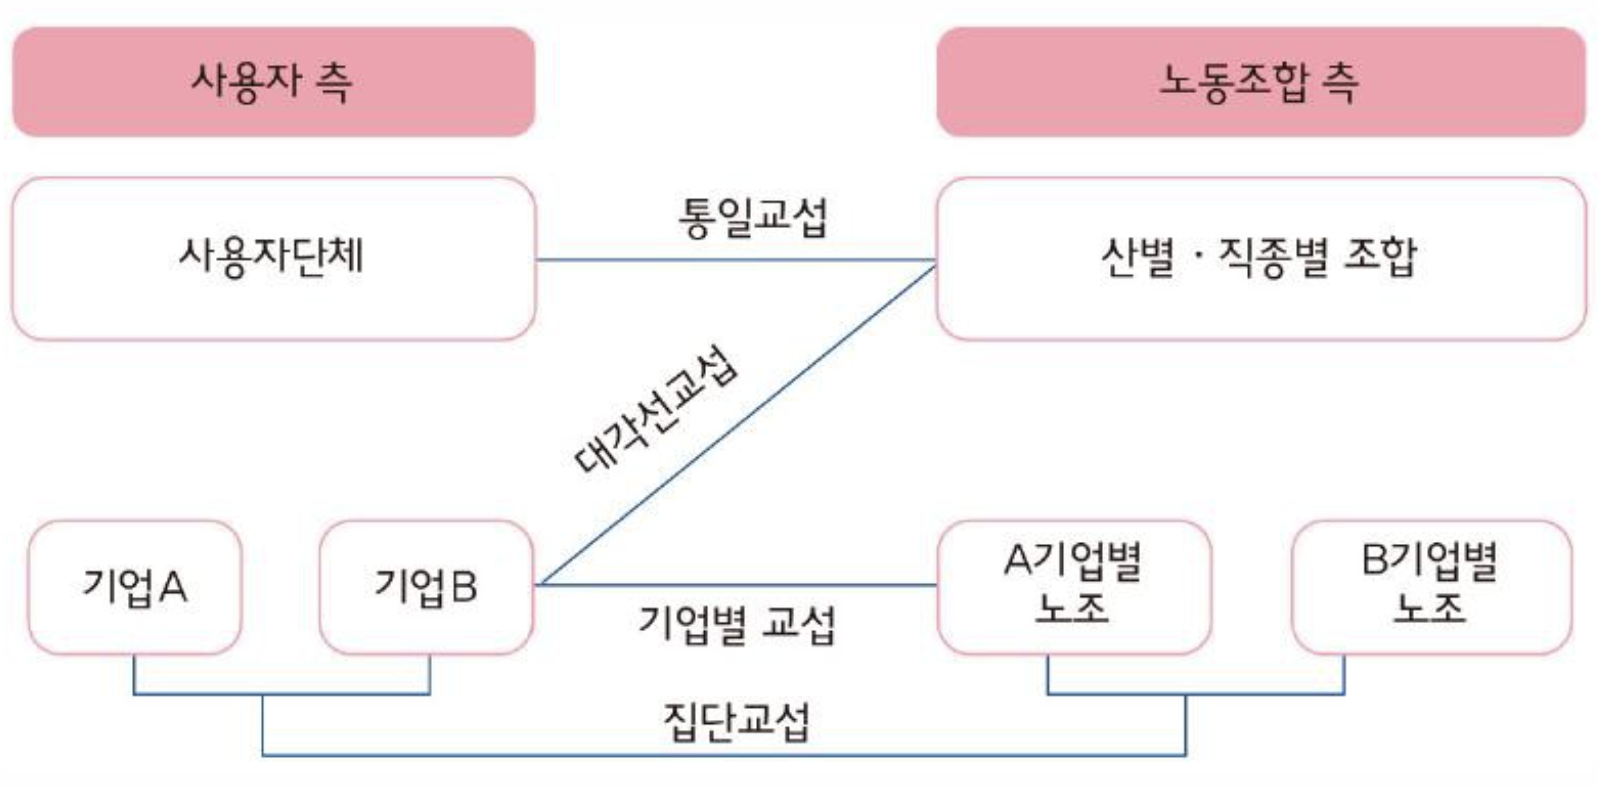
\includegraphics[width=.8\textwidth]{pic/단체교섭유형.png}
        \caption{단체교섭의 유형}
    \end{figure}
\end{frame}

\section{단체교섭의 과정}

\begin{frame}{단체교섭의 순서도}
\centering
\begin{figure}
    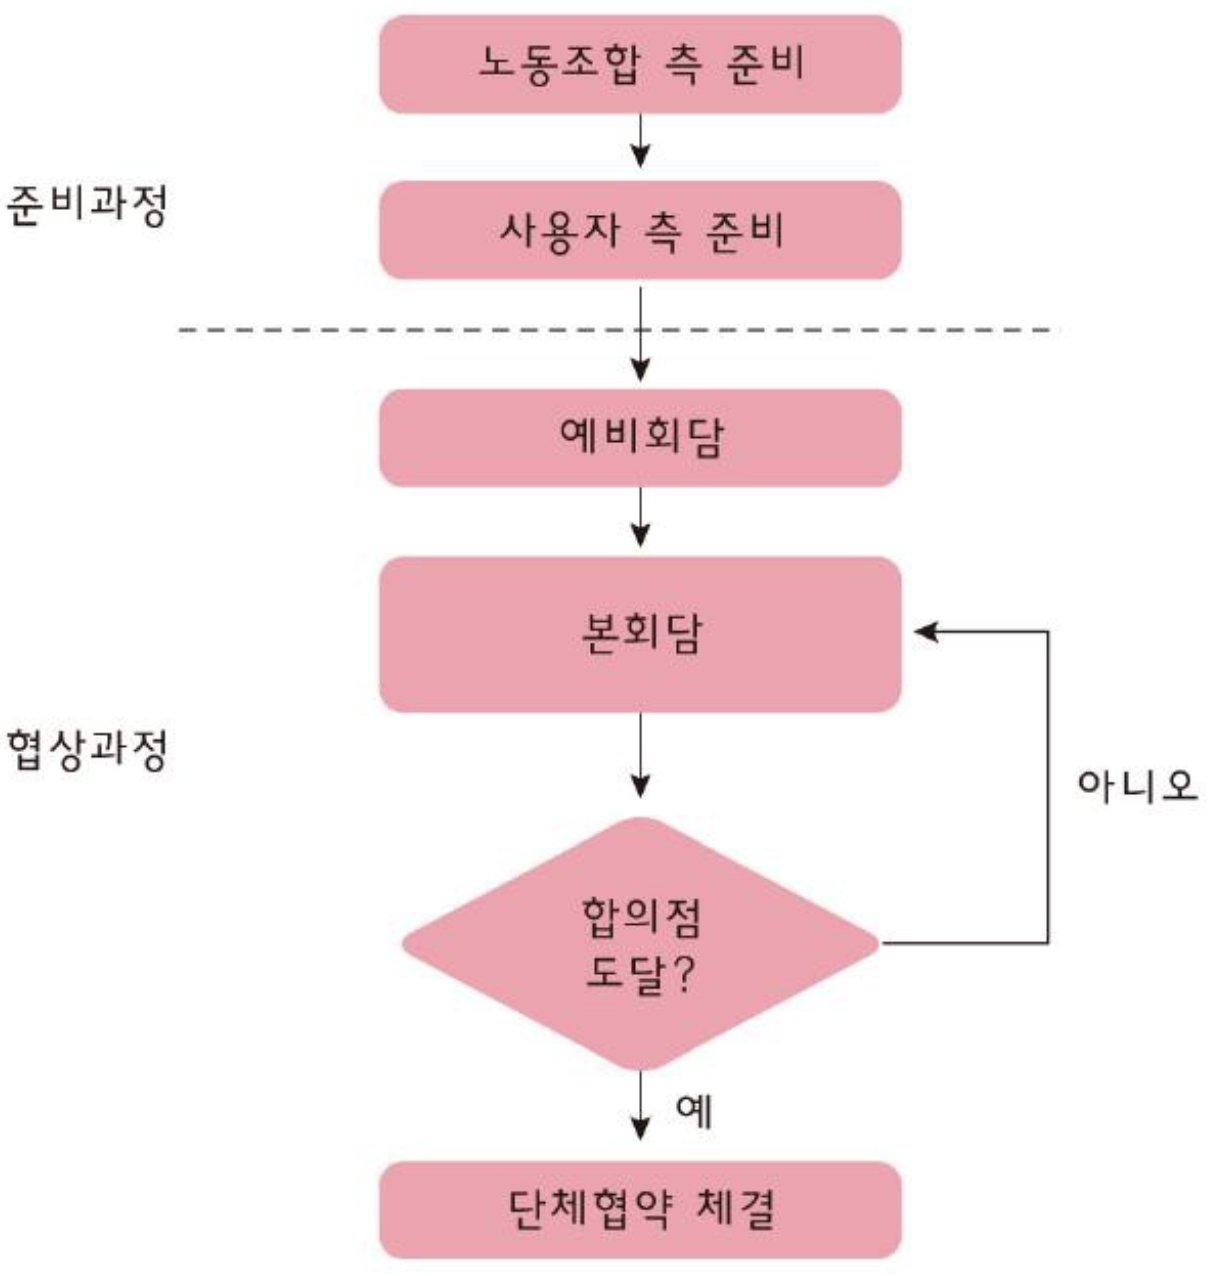
\includegraphics[width=.35\textwidth]{pic/단체교섭절차.png}
    \caption{단체교섭의 절차}
\end{figure}

\end{frame}
\begin{frame}{노조측의 준비사항}
    \begin{itemize}[<+->]
        \item 노동조합은 단체교섭을 위한 요구안 작성
        \item 요구안은 요구사항과 그 배경설명 등으로 구성하되,
        \begin{itemize}[<+->]
            \item 특히 요구사항에 대한 배경자료의 준비 노력 필요 (대외적 명분과 성과 좌우)
            \item 또한 요구수준은 타협가능하고 납득할 수 있는 적정수준으로 설정 필요
        \end{itemize}
    \item 배경자료의 내용: 조합원의 생활실태 및 불만·요구, 동종업체와의 비교, 상위 노조의 지침 등 첨부
        \begin{itemize}[<+->]
            \item 특히, 기업의 경영실적 및 전망 등에 대한 자료 확보 필요
        \end{itemize}
    \end{itemize}
\end{frame}

\begin{frame}{사용자측 준비사항}
    \begin{itemize}[<+->]
        \item 사용자측은 협상 전 노조의 교섭요청항목을 세밀히 검토해야
        \begin{itemize}[<+->]
            \item 노조의 요구사항 및 요구 수용 시 비용 증가액 추산
            \item 또한 사용자측의 요구항목 발굴 필요 
        \end{itemize}
    \item 교섭항목의 선정과 내용분석 후, 상대방을 이해·설득시킬 수 있는 자료 준비, 즉 관계법령, 동종 업체의 상황 및 경제 상황 등을 수집·분석해 두어야 
    \item 교섭담당자는 교섭항목의 우선순위 선정하고 각 항목에 대하여 성취하고자 하는 적정한 목표 설정
    \item 주의할 사항: 노조의 요구안을 반박하는 형식이 아닌 각종 대안과 장기적·연차적인 처리방안 강구
    \end{itemize}
\end{frame}

\begin{frame}{예비회담}
    \begin{itemize}[<+->]
        \item 본격적인 단체교섭에 들어갈 자세 확립
        \begin{itemize}[<+->]
            \item 협상절차 결정
            \item 상호 교섭하고자 하는 항목 교환
            \item 협상의 시기와 장소
            \item 교섭위원의 수 및 자격요건
            \item 단체협약 체결방법 등
        \end{itemize}
    \item 단, 상호 교환된 항목 이외의 사항은 본 협상 진행 중에 제안할 수 없음을 명시할 필요
    \end{itemize}
\end{frame}

\begin{frame}{본 회담의 진행}
    \begin{itemize}[<+->]
        \item 제1차 회담: 쌍방 대표단의 소개, 제안된 항목의 배경설명 및 질의교환 등을 통해 협상분위기 조성
        \begin{itemize}[<+->]
            \item 특히, 첫 회담이므로 대표자가 참석하는 것이 바람직
            \item 또한 쌍방간에 요구사항 및 배경논리 등을 충분히 설명하여야
        \end{itemize}
        \item 제1차 면담 후, 실무교섭을 통한 각 항목별 세부 의견교환
        \begin{itemize}[<+->]
            \item 쌍방간의 이견차이가 작거나 비교적 덜 중요한 항목은 합의나 교환 그리고 이 항목에 대한 합의서 작성
        \end{itemize}
    \item 처리 안된 중요한 사항은 최종 합의에 도달하도록 노력
    \item 특히, 쌍방 모두는 유연성과 인내심을 갖고 상대방의 의견을 청취하여야 (∵협상 결렬 원인의 상당수가 감정상의 문제에서 기인)
    \end{itemize}
\end{frame}

\begin{frame}{합의에 도달}
    \begin{itemize}[<+->]
        \item 최종 합의 후 협약서를 작성하고 서명·날인
        \item 교섭을 진행하며 나타날 수 있는 갈등이나 마찰을 해소하고 평화적 분위기에서 서로 협력하며 협약의 성실한 이행 및 생산성 증대 등에 대한 결의 필요
    \end{itemize}
\end{frame}

\section{단체교섭의 구성요소}

\begin{frame}{내부조직적 교섭 (intraorganizational bargaining)}
    \begin{itemize}[<+->]
        \item 노조의 내부 또는 사용자들의 내부에서 이루어지는 타협 과정
        \begin{itemize}[<+->]
            \item 교섭이 원만하게 타결되기 위해서는 노사 모두 조직내부적인 동의를 필요로 함
        \end{itemize}
    \item 노조측: 다양한 특성을 가진 조합원들의 이해관계를 사전에 조율하고 강력한 교섭력을 확보 위해
        \begin{itemize}[<+->]
            \item 조합원들을 대상으로 한 설문조사, 교섭일정 공개 및 교섭과정의 투명성 확보
        \end{itemize}
    \item 사용자측: 교섭이 이루어지기 전에 부서간, 부처간 내부 조율 즉 내부조직적 교섭이 발생
    \end{itemize}
\end{frame}

\begin{frame}{분배적 교섭 (distributive bargaining)}
    \begin{itemize}[<+->]
        \item 한정된 파이 (pie)의 몫을 분배할 때 이루어지는 전통적인 단체교섭으로 당사자간의 이해관계에 따른 갈등을 해소하기 위한 협상, zero sum 교섭
        \item 노사는 상호의존성을 갖고 있으나 비용측면에서는 상대방을 약화시키기 위해 각종 전술 (예: 노조의 파업, 사용자측의 조업 계속, 직장폐쇄, 허세 (bluffing) 등)을 사용하여 자신의 이익을 극대화
        \begin{itemize}[<+->]
            \item 교섭당사자는 BATNA보다 단체협약안이 바람직하다고 판단될 때 단체협약 수용
            \item cf. BATNA (best alternative to a negotiated agreement): 협상이 파국을 맞을 때의 대안
        \end{itemize}
    \end{itemize}
\end{frame}

\begin{frame}{통합적 교섭 (integrative bargaining)}
    \begin{itemize}[<+->]
        \item 노사공통의 관심사 (예: 생산성 증대, 비용절감, 안전관리 등)에 대하여 노사가 교섭하여 노사 모두 이익을 얻는 교섭 유형. 상호이익협상 (mutual gains bargaining)
        \item 한정된 파이의 몫을 나누는 분배적 교섭과는 달리 파이의 크기를 증대시키기 위한 쌍방간의 노력
        \begin{itemize}[<+->]
            \item 전통적·대립적·분배적 교섭을 대치 및 보완하고 노사 양측이 함께 만족하는 합의안 도출
        \end{itemize}
    \item 공통 관심사를 해결하기 위한 대안 모색 및 도출하여야
        \begin{itemize}[<+->]
            \item brain storming, 쌍방간의 신뢰 구축, 양적·질적 정보 공유 구출 등이 중요
        \end{itemize}
    \end{itemize}
\end{frame}

\begin{frame}{태도적 구성 (attitudinal structuring)}
    \begin{itemize}[<+->]
        \item 노사간의 전반적인 관계를 개선하기 위한 정서적인 교섭
        \item 교섭과정에서 상대방에 대한 개인적 특성 및 경험 등을 알게 됨
        \begin{itemize}[<+->]
            \item 상호간의 신뢰관계 구축 또는 감정의 골이 깊어질 수도
            \item ∵협상대방에 대한 태도는 교섭에서 중요한 역할을 수행
        \end{itemize}
    \item 교섭의 결과물인 쌍방간의 관계를 근간으로 하여 사회적 계약의 형태를 취하게 됨 
    \end{itemize}
\end{frame}

\section{교섭력 이론}

\begin{frame}{교섭력의 정의}
    \begin{block}{교섭력 (bargaining power)}
        노동조합 또는 사용자가 자신의 교섭조건에 동의하도록 상대방을 이끌어 내는 능력
    \end{block}
    \begin{itemize}[<+->]
        \item 단체협상에서 사용자의 교섭력은 노조의 교섭력과 서로 반비례
        \item 노조의 교섭력
        \begin{itemize}[<+->]
            \item 사용자가 고임금과 근로조건 향상을 위해 지불할 수 있는 능력 (employer ability to pay)
            \item 사용자로 하여금 지불하도록 하는 노조의 능력 (union ability to make employers pay)
        \end{itemize}
    \end{itemize}
\end{frame}

\begin{frame}{교섭이론의 개념}
    \begin{figure}
        \centering
        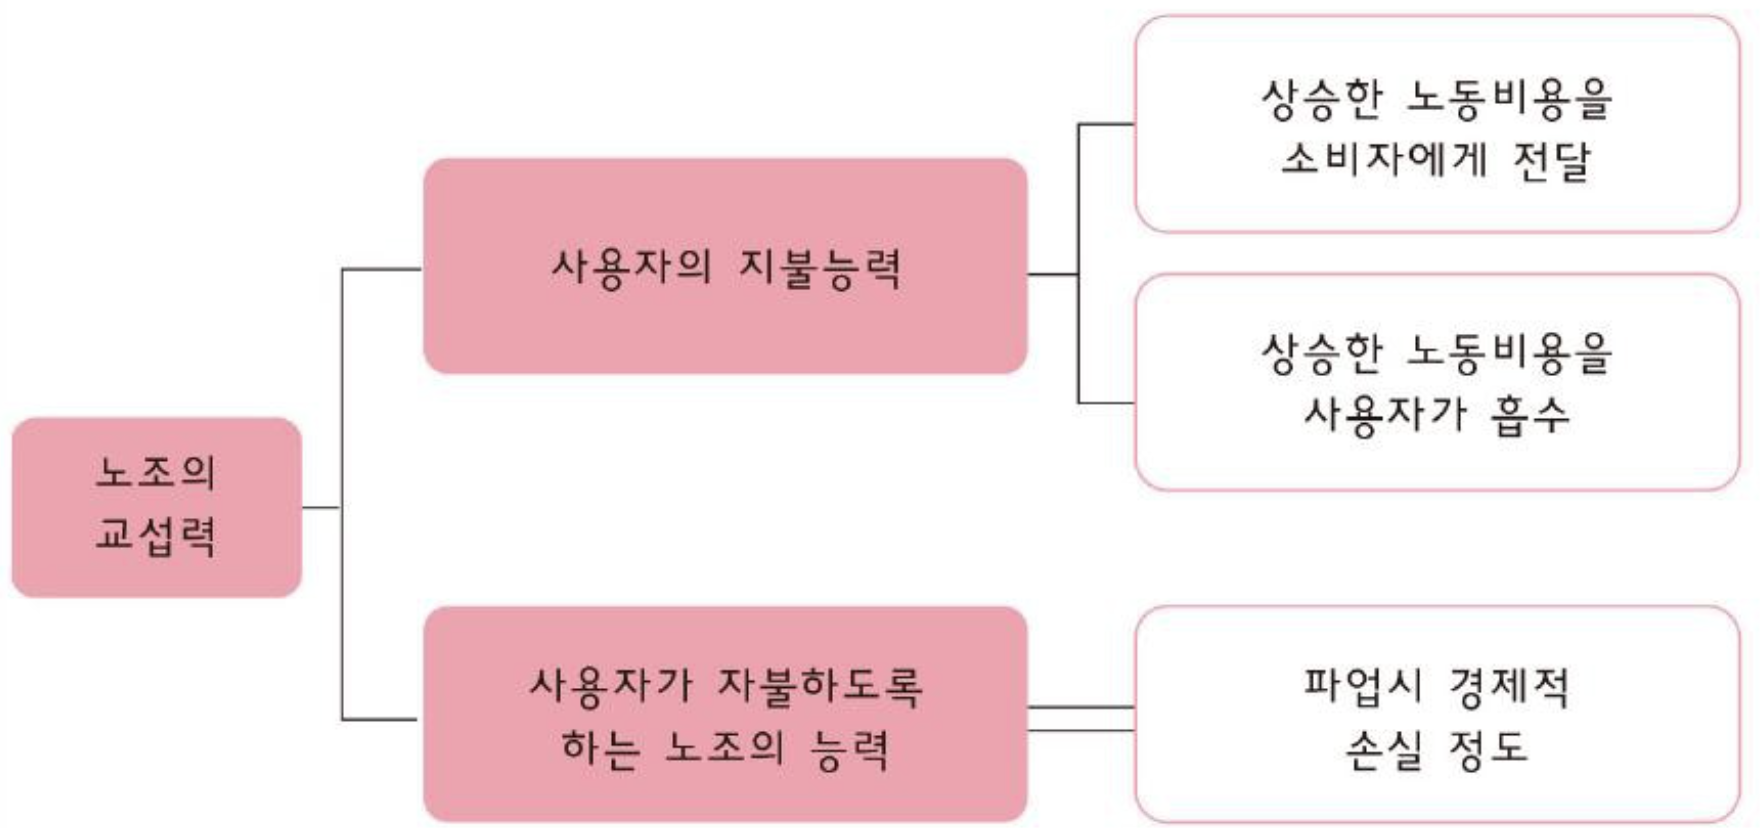
\includegraphics[width=.8\textwidth]{pic/교섭이론의 개념요약.png}
        \caption{교섭이론의 개념요약}
    \end{figure}
\end{frame}

\begin{frame}{사용자의 지불능력}
    \begin{itemize}[<+->]
        \item 사용자의 지불능력: 노조가 요구하는 임금인상이나 근로조건 개선 등을 수용할 수 있는 사용자의 능력으로 다음의 4가지가 일반적임
        \begin{enumerate}[<+->]
            \item 소비자 전가: 노동비용 인상분은 소비자에게 전가할 수 있는 경우
            \item 지역적 제약: 타 지역으로 기업진출이 어려운 경우
            \item 산별 노조: 노조의 교섭력이 강하고 산별 교섭이 이루어지는 경우
            \item 정부 지원: 정부의 지원이 존재하는 경우
            \item 사용자 흡수: 노동비용 인상분은 기업에서 흡수하는 경우
        \end{enumerate}
    \end{itemize}
    \begin{exampleblock}{사용자 흡수의 예시}
        \begin{itemize}[<+->]
            \item 자본집약적 산업에 신규 자본투자를 통한 생산성 증가로 노동비용 인상분을 흡수
            \item 초과이윤을 획득하던 독과점기업이 주주에게 지불되던 초과이윤을 축소
        \end{itemize}
    \end{exampleblock}
\end{frame}

\begin{frame}[allowframebreaks]{노조의 사용자 지불 강제능력}
    \begin{itemize}[<+->]
        \item 노조 교섭력의 원천은 파업위협이며 사용자측 교섭력의 원천은 파업을 억제하는 능력. 즉, 교섭력은 파업으로 인한 우리측의 손실과 상대방측의 손실간의 차이에서 발생
            \[\text{교섭력} = \frac{\text{파업시 상대방의 손실}}{\text{파업시 나의 손실}}\]
        \begin{itemize}[<+->]
            \item 파업으로 인한 노조측의 손실이 작다면 노조측의 교섭력이 사용자측보다 강하기 때문에 영향력이 큼 (반대의 경우도 성립)
            \item 여기서의 손실이란 단순히 경제적 손실뿐만 아니라 정부와 소비자의 압력, 여론의 부정적 동향 등을 포괄하는 의미
        \end{itemize}
        \item 생산품의 내구성이나 유형: 석탄, 철강제품 등 내구성이 있는 제품은 노조의 파업 위력이 약함 (반대 경우도 성립)
        \item 수직적 계열화 회사의 경우: 파업으로 연관회사에 큰 타격: 노조 교섭력이 상대적으로 강함 
        \item 노조와 노조원의 구성상 특징과 성격: 노조원 중 회사 핵심인력의 포함 여부, 산업 내 다른  노조의 존재 여부
        \item 노동집약적 산업: 노동력이 중요하기 때문에 노조 교섭력 강함 (반대의 경우도 성립)
        \item 경제적 여건: 호경기에 사용자는 매출 호기를 잃어버리기 때문에 노조의 파업 위력 강함 (반대의 경우 성립)
        \item 교섭구조: 산업별 교섭이 기업별 교섭보다 노조의 규모가 커져 노조의 교섭력 강함
        \item 노조나 사용자의 투쟁력이나 단결력이 강하면 상대방에 대하여 상대적으로 강한 위력
        \item 파업에 대한 정부 규제
        \item 사용자에게 타격을 주기 위한 여러 방안: 보이콧, 태업 등, 사용자는 파업보험 가입 여부
    \end{itemize}
\end{frame}

%------------------------------------------------
\end{document}
%------------------------------------------------
